\section{Introduction}

% [cite{LDB, Medprompt, MetaGPT, xxx to be added}]
% Professionally designed workflows bring Large Language Models (LLMs) to stronger capabilities and wider application scenarios. \yuyu{I think we should ``copy'' this sentence as the beginning of the Abstract.} \mc{should first define what SOP is and what workflow is. Or they are the same? It is vague to ignore this in title/abstract/intro.}

Professionally designed workflows bring Large Language Models (LLMs) to stronger capabilities and wider application scenarios.

% 第一段引出workflow与agent，说明agentic workflow与动态的agent的差异

% 第二段引出SOP，说明llm agentic workflow的思想在人类社会中一直就有。我们认为优化Workflow的过程可以被认为是人类获取SOP的过程，使用SOP地概念来表示这个新的问题。因为他们面临一样的困境，就是需要消耗大量的Human Cost

% 第三段引出，从automl的历史来看，这种大量的人工设计是不合理的，sop的获取需要自动化实现，这因此带来一个问题，我们应该如何表示SOP的获取问题？提出这个问题是因为现有的工作往往关注在agentic workflow的单独的方面，比如prompt，contrlflow，hyperparameters，还没有人为SOP的获取给出一个完整的问题定义，也就无从实现探索SOP的自动获取

% 第四段引出，基于这个Motivation，我们提出了一个简单但全面的使用node组织sop的结构，定义了sop优化的全流程，包括node，control flow,workflow，evaluation，optimial process,与sop。通过对过去工作的分析发现，不同方法在做SOP的自动获取时，实际上存在着一个权衡，也就是人工设计越高，搜索效率越高。这显然不能有效的大面积推广，我们基于这个Motivation，提出了SOPtimizer，通过less human design，实现了better的搜索效率

% 介绍SOPTimizer的方法

% 介绍SOPTimizer的实验效果

Recent research \cite{li2024debug} shows that weaker LLMs (e.g., GPT-4o mini, Deepseek-chat) combined with domain-specific Standardized Operating Procedures (SOPs) can outperform stronger LLMs (GPT-4o, Claude 3.5 Sonnet) in multiple domains. For both researchers and engineers, the challenge in utilizing agentic workflows lies not in building them, but in making them effective. The latter often demands that experts convert human-oriented SOPs (Standard Operating Procedures) into agent-oriented workflows, followed by extensive validation to produce reliable Agentic SOPs. As Foundation Models continue to evolve, some handcrafted workflows may require redesign, which negatively impacts the efficiency of agents in real-world applications.
\yuyu{Are there any existing works that use human-crafted SOPs?} \mc{MetaGPT}

\begin{figure}[t!]
  \centering
  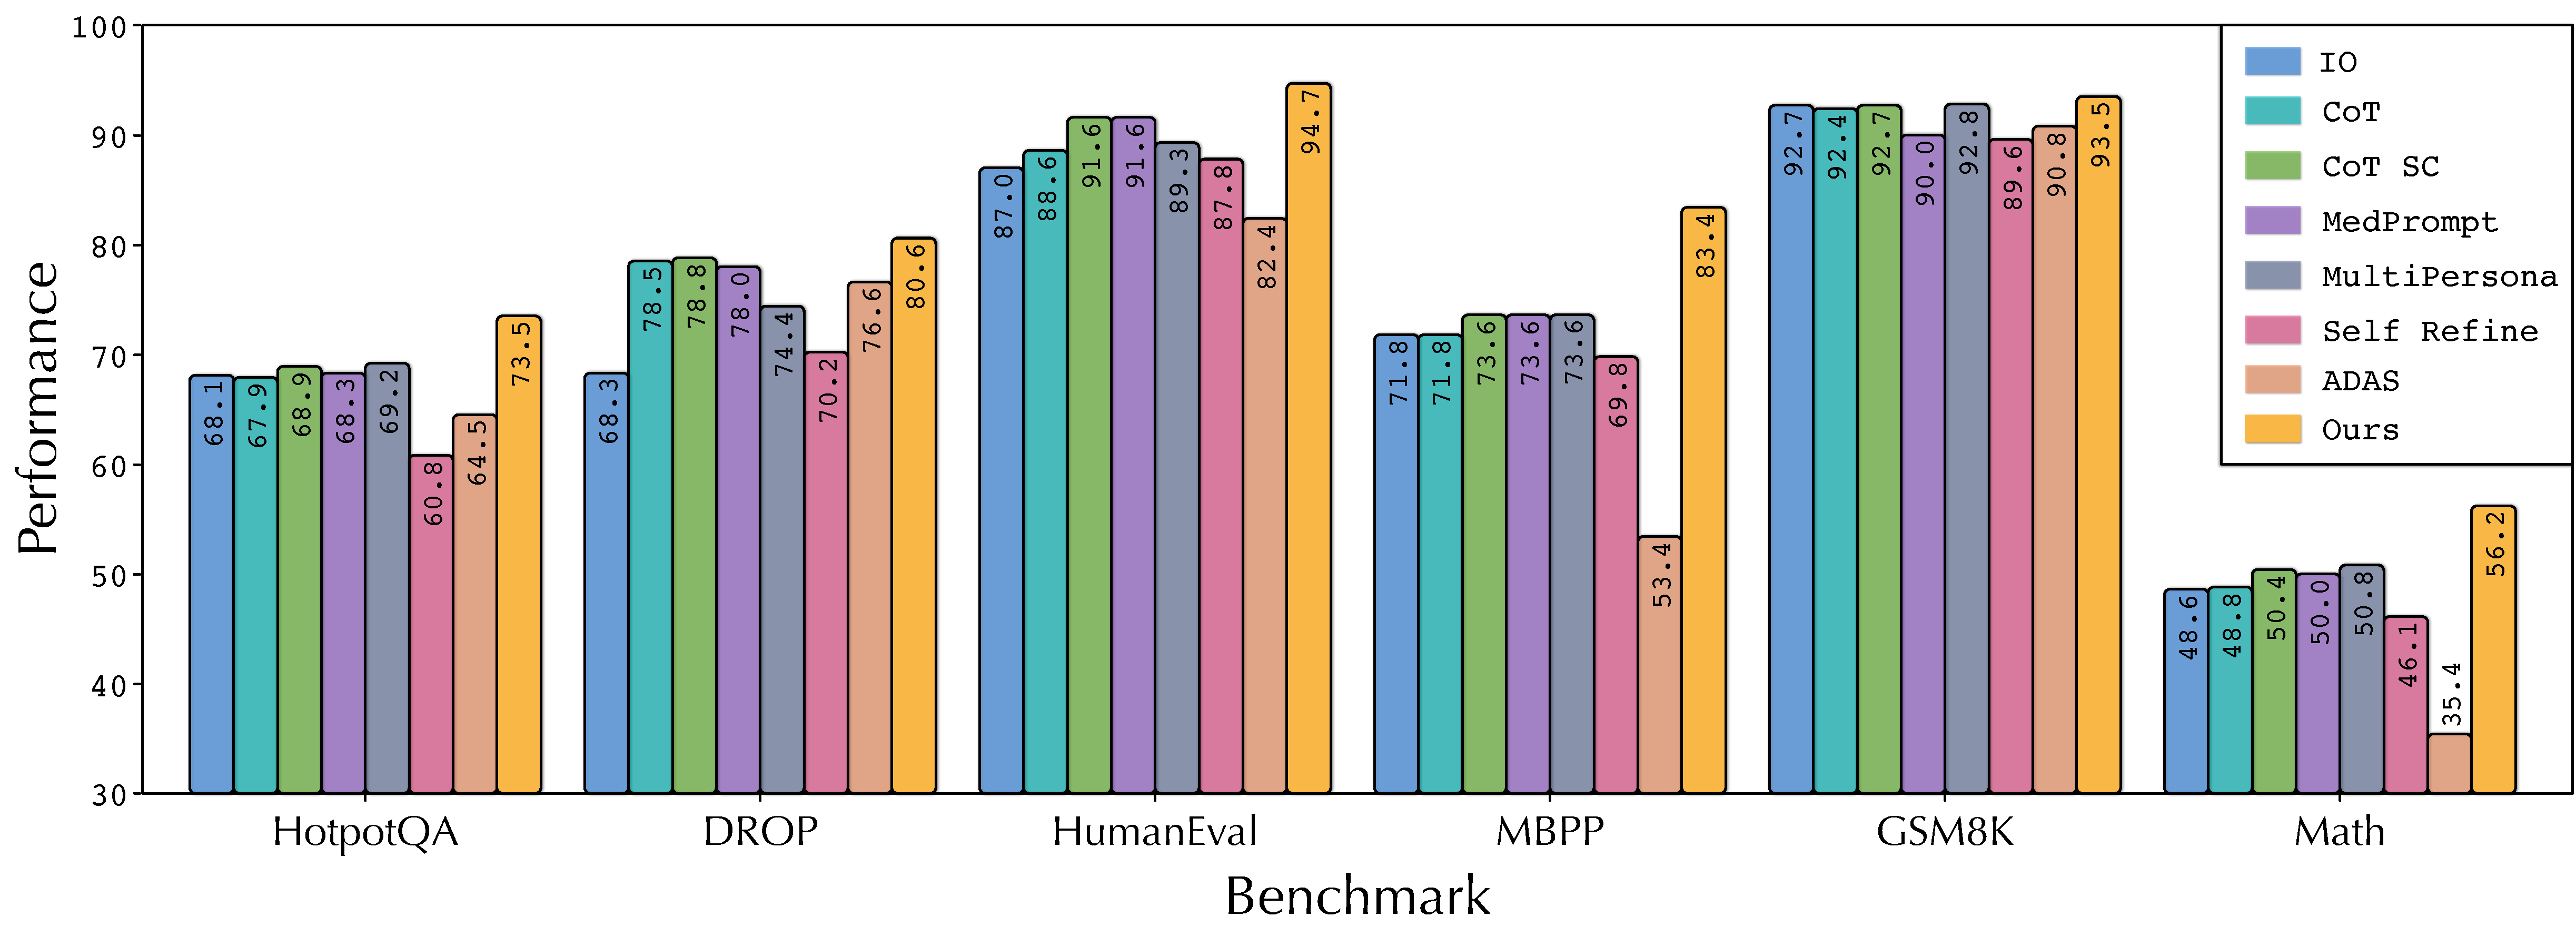
\includegraphics[width=\linewidth]{images/group_bar.pdf}
  \label{pareto front}
  \caption{Comparison Between A And B}
\end{figure}

Recent works \cite{mert2024text, cheng2024opro, chirs2024prompt, xin2024prompt} attempt to solve this problem through automatic prompt optimization. By using a fixed workflow, they perform independent or joint feedback-based optimization for prompts at specific nodes. However, for most scenarios, optimization at the prompt level lacks adaptability of process and therefore struggles to achieve optimal solutions. Optimizing both prompts and workflows shows promise in better addressing this issue. Based on this insight, \cite{hu2024automated, wang2024symbo, zhuge2024gptswarm} explore automatic generation and optimization of workflows, representing workflows in forms such as graphs, computation graphs, and code, and optimizing both prompts and workflows through reinforcement learning, back-propagation, and environmental feedback.  
% SOP强调 -> SOP进展 -> 再说在什么任务上做优化 -> 不存在完全自动的过程xxxx -> 我们提出了一个优化器 

% \yuyu{summarize the limitations of \cite{hu2024automated, wang2024symbo, zhuge2024gptswarm}  in a sentence.}

Despite these advancements, there remains significant room for improvement in the automatic acquisition of domain-specific effective workflows i.e., SOPs. This gap is largely due to differing perspectives on the representation and optimization methods for agentic workflows. Using graphs to represent agentic workflows has certain limitations. For example, when dealing with complex workflow processes, graphs struggle to represent IF-ELSE control flows, and describing them as state machines sacrifices system determinism. Consistent with \cite{hu2024automated}, we posit that code is the most effective representation for agentic workflows. Code is a superset of graphs, theoretically retaining the advantages of graph representations while more flexibly integrating control flows and logical reasoning, thereby addressing the shortcomings of graph-based approaches. However, what truly hinders current work from moving towards automatic acquisition of SOPs is the optimization method for agentic workflows. The approach used by \cite{hu2024automated} lacks well-defined optimization principles, relying instead on simple experiential learning (analog learning) and random sampling, moving it far from obtaining effective workflows.
\yuyu{The discussion of the limitations of existing work is redundant and should be concise.}

\yuyu{This paragraph is hard to follow. Why does our method work? You can list the main points so I can revise them.}
By atomizing the Critical Thinking, we derive a reliable representation for acquiring agentic SOPs, which we call SOPtimizer. We represent the atomized actions as Operators and refer to the workflow that represents the logical relationships between operators as a SolveGraph in code form. SOPtimizer atomizes the workflow of general tasks, deriving 10 basic operators. Subsequently, given a dataset, SOPtimizer analyzes and questions the completeness and reliability of the existing set of operators for that dataset, and through cycles of verification and refinement, obtains domain-specific optimized operators. With an effective foundation established, SOPtimizer then uses performance and cost as the optimization objective, conducting cycles of analysis, questioning, verification, and refinement on the structure of the SolveGraph. This approach ensures effective optimization and rapid convergence by adhering to a traceable and logical optimization process.

To validate the effectiveness and generalizability of SOPtimizer in acquiring agentic SOPs, we conducted quantitative experiments in logical reasoning scenarios (code, math, question answering), comparing it with General Agents, workflows obtained by similar works, and domain-specific workflow state-of-the-art (SOTA) methods. We also performed case studies in daily task scenarios (writing, vision) to verify its impact on the real world. The quantitative experimental results demonstrate that the agentic workflows automatically acquired by SOPtimizer significantly outperform handcrafted general agents and workflows discovered from similar works. On the GSM8K dataset, it achieved 95.6\%, just 2.5\% behind the SOTA which required substantial effort. On MATH, HumanEval, MBPP, HotPotQA, and DROP datasets, it exceeded over 95\% of the current SOTA scores, effectively validating the effectiveness of agentic workflows and thus achieving automated SOP acquisition. In the performance-oriented SOP acquisition process, SOPtimizer also discovered cost-oriented SOPs. In comparison with other methods, it maintained Pareto optimality across 6 datasets. Figure \ref{pareto front} illustrates these results.

We summarize the contributions of this paper as follows:

\begin{itemize}
    \item We identify key obstacles (workflow and effective workflow) ...
    \item We introduce critical thinking as a meta-optimization methods ...
    \item We introduce SOPtimier, acquiring SOPs in logic reasoning sceniros ... 
\end{itemize} 